
% Please note that whilst this template provides a 
% preview of the typeset manuscript for submission, it 
% will not necessarily be the final publication layout.
%
% letterpaper/a4paper: US/UK paper size toggle
% num-refs/alpha-refs: numeric/author-year citation and bibliography toggle

%\documentclass[letterpaper]{aejstyles}
\documentclass[a4paper,alpha-refs]{eSpectra}
\usepackage[utf8]{inputenc}
%%% Journal toggle; only specific options recognised.
\journal{aej}

\usepackage{graphicx}
\usepackage{siunitx}
\usepackage[spanish, english]{babel} % Spanish for default (Abstract. References, Appendix, tables, and figures names).
\usepackage{amssymb}
\usepackage{comment}

\setcounter{page}{22}

\usepackage{hyperref}
\usepackage{academicons}
\usepackage{aas-macros}
\usepackage{doi}
\usepackage{fontawesome5}
\usepackage[left]{lineno}

\renewcommand{\doitext}{}


\definecolor{orcidlogocol}{rgb}{0.65, 0.807, 0.223}
\newcommand{\orcid}[1]{$\,$\href{https://orcid.org/0000-0001-7868-9934}{\textcolor{orcidlogocol}{\faOrcid}}}
 
%\usepackage[left]{lineno}
%\linenumbers

%%% Flushend: You can add this package to automatically balance the final page, but if things go awry (e.g. section contents appearing out-of-order or entire blocks or paragraphs are coloured), remove it!
% \usepackage{flushend}


\title{El Observatorio Solar de Bacatá: Nuevas perspectivas Arqueo-astronómicas en el centro histórico de Bogotá.}

%%% Use the \authfn to add symbols for additional footnotes, if any. 1 is reserved for correspondence emails; then continuing with 2 etc for contributions.
\author[1]{Usuy D. Leon Tolosa\authfn{1}}
\author[2,3]{Jaime E. Forero-Romero\authfn{2}}
\affil[1]{Universidad Nacional de Colombia, Bogotá D.C., Colombia}
\affil[2]{Departamento de Física, Universidad de los Andes, Cra. 1 No. 18A-10, Edificio Ip, CP 111711, Bogotá, Colombia}
\affil[3]{Observatorio Astronómico, Universidad de los Andes, Cra. 1 No. 18A-10, Edificio H, CP 111711 Bogotá, Colombia}

%%% Author Notes
\authnote{\authfn{1} Biologo - Investigador (udleont@unal.edu.co)}
\authnote{\authfn{2} je.forero@uniandes.edu.co }


%%% Paper category: Other categories include: Research Article, Review, News, Announcements, Interviews, Opinion, Resources & Activities, Book Review, Correspondences, Best practice,
\papercat{Scientific Article}

%%% "Short" author for running page header
\runningauthor{Leon et al.}

%%% Should only be set by an editor
\jvolume{2}
\jnumber{1}
\jyear{2024}
\begin{document}
\begin{frontmatter}
\maketitle

\selectlanguage{english}
\begin{abstract}
\justifying
The previous existence of a Solar Muisca Observatory in Bacata, located at the current site of the Primada Cathedral in Bogotá, is a widely disseminated hypothesis in popular culture, suggesting that the Muisca people observed alleged solar alignments during the solstices and equinoxes, when the sun emerges over the surrounding mountains. Although historical records indicate that European friars marked indigenous sacred sites with crosses, and churches were later built on some of these sites, the specific claim regarding the Cathedral lacks rigorous astronomical verification. In this paper, we present calculations indicating that, among all the historic churches in the area, the location of the Cathedral does not show the best alignment with the theoretical observation point, which would be located closer to the Plazoleta del Chorro de Quevedo, historic site that gave rise to the city of Bogotá.

\end{abstract}

\qquad\quad\textbf{Keywords:} Horizon Calendars, Archaeoastronomy, Solar Observatory, Cultural Syncretism.
%------------------------------------------------------------
\selectlanguage{spanish} 
\begin{abstract}
\justifying
La existencia previa de un Observatorio Solar Musica en Bacata ubicado en la posicion actual de la Catedral Primada de Bogotá, es una hipotesis amplimente diseminada en la cultura popular, sugiriendo que el pueblo Muisca  observaba presuntos alineamientos solares durante los solsticios y equinoccios, cuando el Sol emerge sobre las montañas circundantes. Si bien los registros históricos indican que los frailes europeos marcaron sitios indígenas sagrados con cruces, y posteriormente se construyeron iglesias en algunos de estos lugares, la afirmación específica respecto a la Catedral carece de verificación astronómica rigurosa. En este trabajo presentamos cálculos indicando que, entre todas las iglesias históricas del área, la ubicación de la Catedral no muestra el mejor alineamiento con el punto teórico de observación, el cual se encontraría situado mas cerca de la Plazoleta del Chorro de Quevedo, sitio histórico antiguo que dio origen a la ciudad de Bogotá.
\end{abstract}

\begin{skeywords}
Calendarios Horizonte: Arqueoastronomía, Observatorio Solar, Sincretismo Cultural.
\end{skeywords}
\end{frontmatter}
%------------------------------------------------------------
\selectlanguage{spanish} 

\section{Introducion}

La concepción del tiempo para la cultura muisca estaba profundamente relacionada con la observación del dios sol «Xué» y la luna «Chia». Así como con los ciclos de lluvias y sequias anuales de la Sabana de Bogotá \cite{langebaek_muiscas_2005}. Los xeques, observaban cuidadosamente el movimiento de los astros para determinar momentos como el inicio de la temporada de lluvia (entre marzo y abril, cercana al equinoccio de primavera y el inicio de la sequía entre diciembre y enero, coincidente con el solsticio de invierno).  Estas observaciones estuvieron involucradas en la estructura de organización agrícola, permitiendo identificar los periodos propicios para la siembra y la cosecha del maíz y otros cultivos esenciales \cite{duquesne_calendario_acosta_1848}.

El término «calendario de horizonte» designa los sistemas de medición del tiempo basados en la observación de la posición aparente del sol, al amanecer o al atardecer, con respecto a puntos fijos del horizonte natural, como estructuras o cadenas montañosas. En contextos cercanos al ecuador, donde la variación estacional en la duración del día es mínima, estos marcadores geográficos permitieron a las comunidades indígenas determinar con precisión los extremos solares (solsticios) y los puntos medios (equinoccios), que sirven como referencia para un calendario anual \cite{quijano_astronomia_2021}. En el paisaje de la Sabana de Bogotá, el arte rupestre de las comunidades muiscas constituye una evidencia material directa de su observación astronómica. Investigaciones arqueológicas han identificado pictogramas con motivos circulares rodeados de líneas radiadas y figuras zoomorfas interpretadas como representaciones del Sol \cite{munoz_animales_2009, martinez_manual_2004}. Curiosamente, en la sabana de Facatativá y Soacha, las figuras solares aparecen grabadas junto a imágenes de ranas \cite{saenz_cepeda_2020}. Algunos autores resaltan la importancia del sonido del canto de las ranas durante sus momentos reproductivos como indicador de siembra para el pueblo muisca \cite{duquesne_calendario_manuscript_1795}. Considerando que las especies de la sabana como \textit{Rhinella humboldti}  y  \textit{Hypsiboas crepitans} , poseen momentos reproductivos y picos de actividad fijos \cite{cortes_gallo_ecologia_reproductiva_2024}, siempre asociados al inicio de la estación lluviosa de los meses de marzo-abril (mes de equinoccio de primavera). Podríamos sugerir una integración territorial que relacione ciclos solares, lluvias e indicadores biológicos, todos componentes previamente descritos dentro la cosmovisión y arte rupestre muisca. 

\smallskip
\centering
   \includegraphics[width=0.5\textwidth]{images/bitmap.png}
\captionof{figure}{ Pictogramas de la sabana de Cundinamarca (facatativa): Las formas representadas corresponden a diseños de soles y formas zoomorfas, especialmente raniformes. Adaptado de \cite{saenz_cepeda_2020}} 
\justifying

\smallskip

Para integrar estas relaciones territoriales hace falta de un observatorio solar en la sabana de Bogotá, que hubiera sirvido a manera de calendario de horizonte. Previamente su existencia ha sido propuesta usando como referencia las montañas de Guadalupe y Monserrate \cite{bonilla_observatorio_2011}. Al observar dichas montañas desde un área específica en el centro histórico de la ciudad, se puede ver el amanecer del sol desplazarse por diferentes puntos del horizonte. Dicha estrella realiza un aparentemente recorrido de sur a norte y de norte a sur. Donde sus puntos máximos de desplazamiento son los solsticios, y los momentos en que el Sol está a la mitad de su camino los equinoccios. El tiempo de este recorrido constituye un año de 365 días aproximadamente \cite{quijano_astronomia_2021}. Los puntos maximos de este recorrido serian entoces puntos de referencia,  quiza sagrados cercanos al pico de las dos montañas.  Algunos autores describen que previo a la construcción de ermitas cristianas en estos picos , los frailes europeos habían señalado las cumbres con cruces como marcadores de los antiguos "santuarios indígenas" \cite{rodriguez_freyle_carnero_1997}. Los “santuarios” a lo largo del altiplano correspondían a todos aquellos montes, cumbres, fuentes, y  aguas... peñascos donde tenían noticias que los muiscas depositaban figuras y tributo en muchos casos envueltos en algodon  \cite{simon_noticias_historiales_1626}. La posterior construcción de iglesias en estos sitios sagrados culminó el proceso de sincretismo entre la astronomía ancestral muisca y la religión católica.


En el presente trabajo,  utilizamos la ubicación actual de las iglesias de Guadalupe y Monserrate como puntos de geo-referencia para calcular la posición ideal de observación solar durante los equinoccios y solsticios. Mediante el análisis de los ángulos teóricos del azimut solar para estas fechas astronómicamente significativas, determinamos el área óptima para las observaciones solares. Nuestros cálculos revelan que esta área no corresponde a la Plaza de Bolívar, como se acepta actualmente, sino que se localiza con mayor aproximacion a otro sector del centro histórico bogotano: la zona del Chorro de Quevedo en La Candelaria. Adicionalmente, evaluamos la proximidad angular de las seis principales iglesias históricas del centro de Bogotá respecto a los ángulos ideales de observación. Estos hallazgos sugieren nuevas implicaciones para el entendimiento del sincretismo cultural y el desarrollo del astroturismo en la capital colombiana.

%------------------------------------------------------
\vspace{-\baselineskip}  % Elimina una línea de espacio
\justifying
\section{Metodos}

\subsection{Definición de Cordenadas}
\justifying
Se selecciónaron de 8 ubicaciones  de iglesias, ermitas y parroquias  históricas de Bogotá, Todas con inicio de costruccion en los primeros 100 años de la fundacion de la ciudad.

\centering
   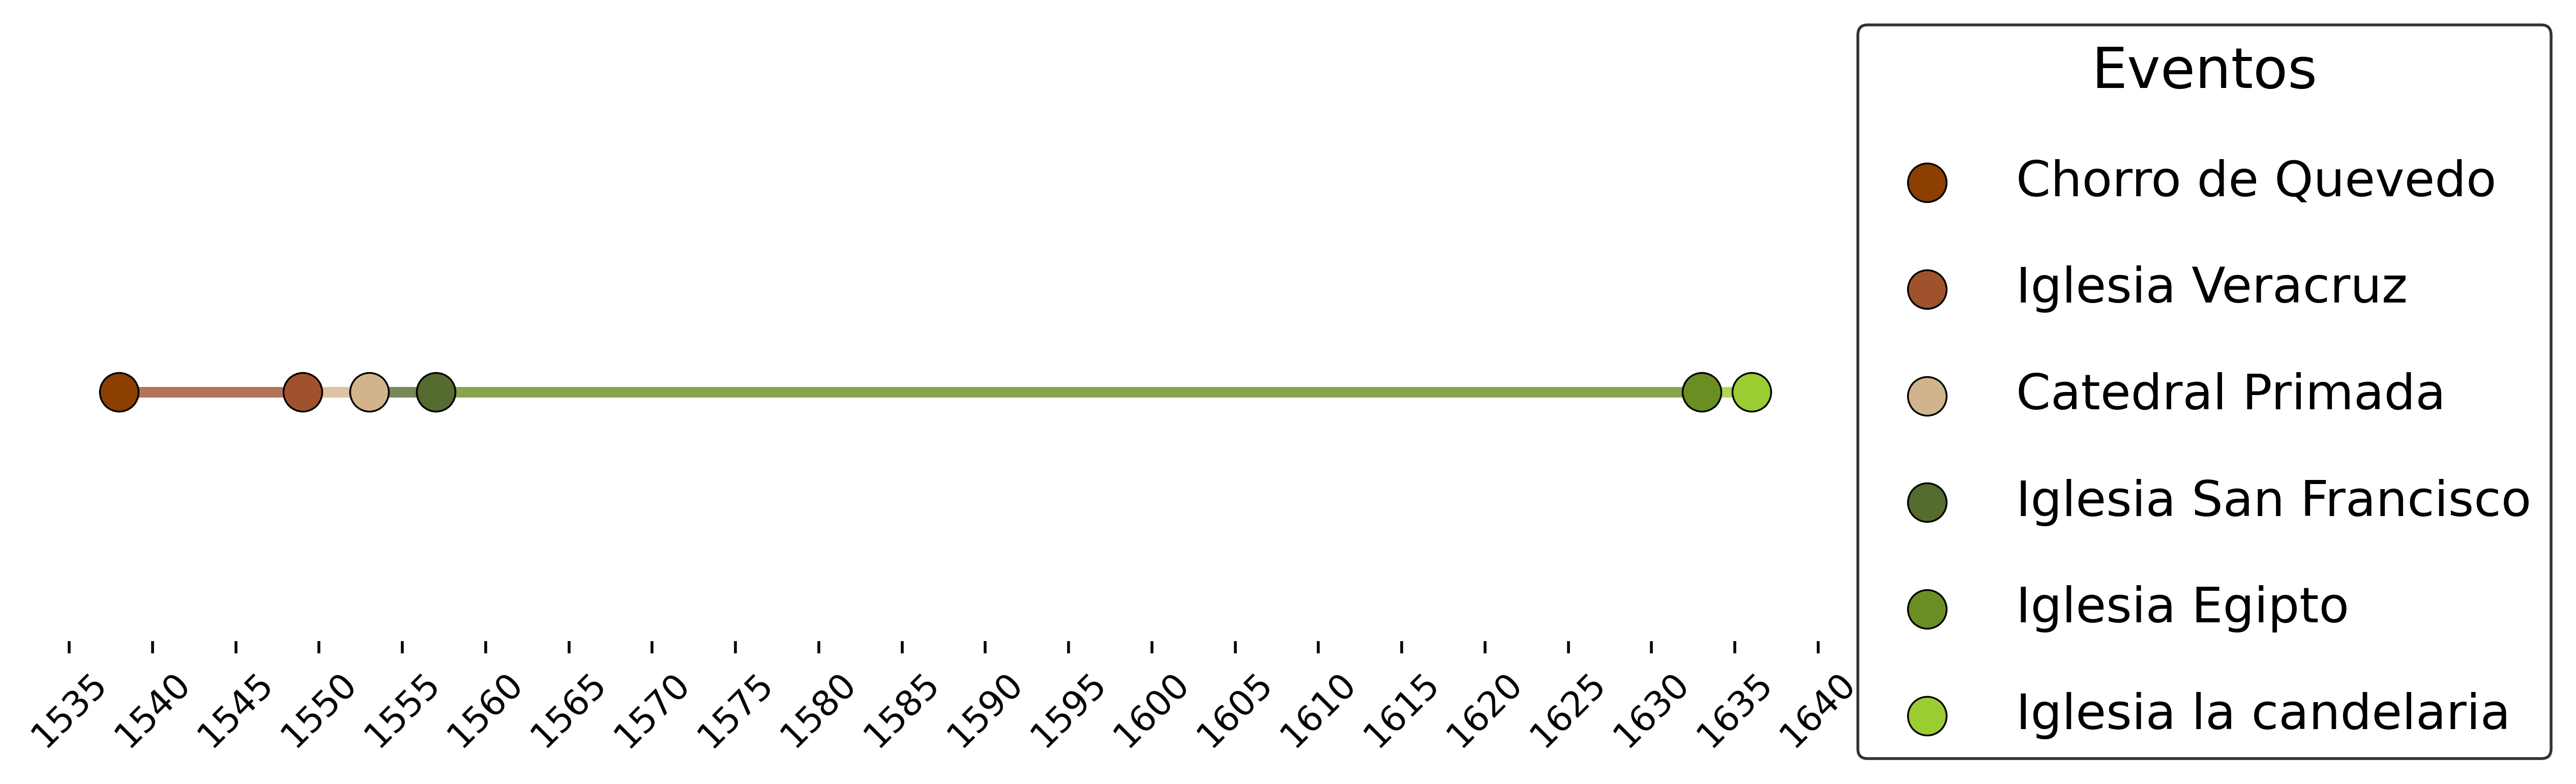
\includegraphics[width=0.5\textwidth]{images/timeline_events.png}
\captionof{figure}{ Linea de tiempo de inicio de construccion de lugares hiistoricos del centro de Bogota. }

\justifying
Especificamente  la Iglesia de nuestra señora de la Candelaria, La parroquia de nuestra señora de Egipto, La iglesia de veracruz, La ermita de san miguel del principe, La catedral primada, y La catedral de San Carlos. 
Para cada uno de estos sitios se definieron coordenadas  GPS ( con una incertidumbre de 7m) , abarcando latitud, longitud y altitud. Las cordenadas fueron usadas para crear 8 triangulos siempre usando como puntos fijos de referencia La ubicacion de la basilisca de nuestro señor de monserrate y La ermita de nuestra señora de guadalupe. Adicionalmente, se calculo un triangulo ideal que estuviera compuesto por los angulos de azimuth ideales cada los solsticios de invierno y de verano, y con puntos fijos en las iglesias de monserrte y guadalupe.

\centering
   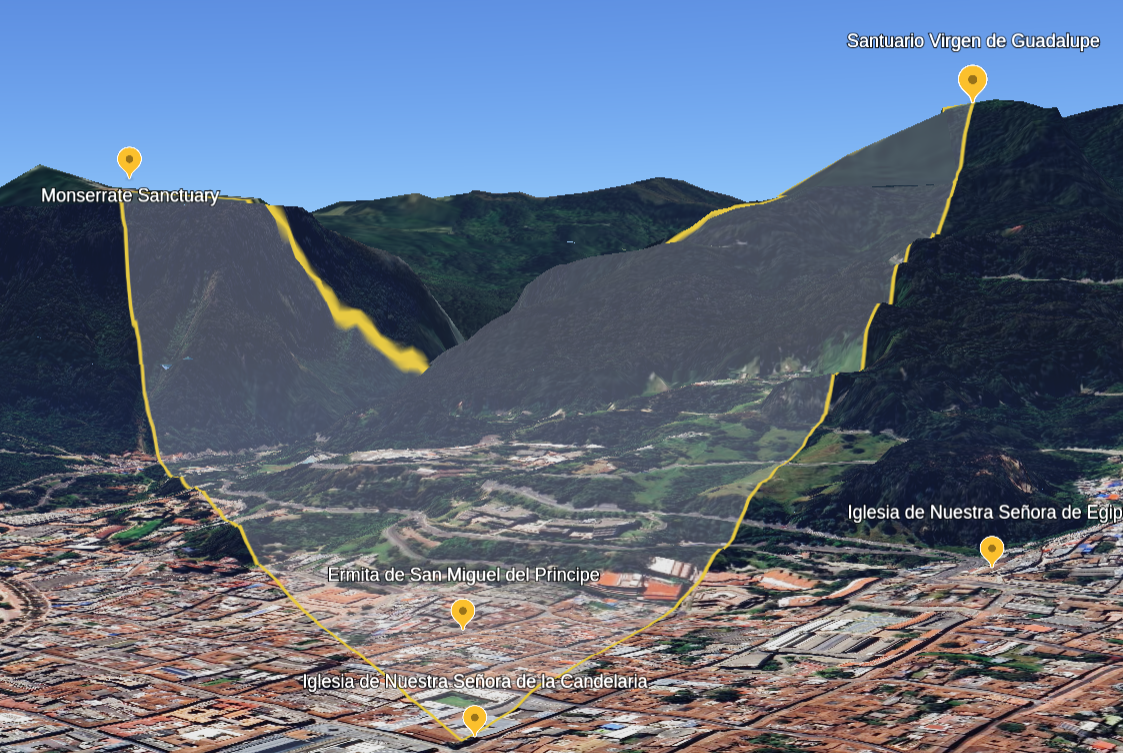
\includegraphics[width=0.5\textwidth]{images/Pasted image 20250617164513.png}
\captionof{figure}{ Alineamientos de los puntos geograficos de centros historicos de bogota respecto a los cerros de guadalupe y monserrate, elaborado en Google earth software. }
\justifying


\subsection{Calculo Azimuth Solar}


\[Azimuth=\arctan \left(
\frac{\sin(H)}{\cos(H)\sin(\varphi) - \tan(\delta)\cos(\varphi)}
\right)\]
\noindent \(H\)= ángulo del Sol, \(\varphi =\) Latitud , \(\delta = \pm 23.44^\circ\): Declinación solar.

\begin{table}[h!]
\centering
\begin{tabular}{|c|c|c|}
\hline
\textbf{Fecha} & \textbf{Azimut}  & \textbf{Dirección} \\ \hline
Equinoccio & 90.0° & Este \\ \hline
Solsticio de verano & 67.1° & Noreste \\ \hline
Solsticio de invierno & 67.2° & Sureste \\ \hline
\end{tabular}
\caption{Angulos Ideales de observacion de salida del Sol}
\end{table}

\vspace{-\baselineskip}  % Elimina una línea de espacio
\vspace{-1\baselineskip}  % Elimina media línea

\subsection{Transformación de Coordenadas Geodesicas}
Para garantizar la precisión en los cálculos, las variaciones topograficas en altura, asi como la curvatura terrestre fueron consideradas, usandose un sistema cartesiano geocéntrico (ECEF). Para convertir la latitud, longitud y altura   \((\varphi, \lambda, h)\) , se utilizan las siguientes ecuaciones:

2. Transformación a coordenadas ECEF

\[
\begin{aligned}
X &= (R + h) \, \cos(\varphi_{\text{rad}}) \, \cos(\lambda_{\text{rad}}) \\
Y &= (R + h) \, \cos(\varphi_{\text{rad}}) \, \sin(\lambda_{\text{rad}}) \\
Z &= (R + h) \, \sin(\varphi_{\text{rad}})
\end{aligned}
\]

- \(X, Y, Z\) son las coordenadas cartesianas ECEF (en km).

- \(R\) es 6371 km el radio medio terrestre.


%------------------------------------------------------------

\subsection{Cálculo de Ángulos}
Para calcular los ángulos interiores de cada triángulo en el espacio tridimensional se computó vectores entre los puntos transformados mediante operaciones de resta vectorial, determinó el producto punto entre estos vectores y se normalizó por sus magnitudes respectivas.  Culminando con la conversión final del ángulo resultante de radianes a grados para su interpretación geométrica.

\smallskip

Para los tres puntos en el espacio:
\[
A(x_1, y_1, z_1), \quad B(x_2, y_2, z_2), \quad C(x_3, y_3, z_3)
\]

Los vectores formados son:
\[
\vec{AB} = \vec{B} - \vec{A}, \quad
\vec{AC} = \vec{C} - \vec{A}
\]

El ángulo en el vértice \(A\) se calcula mediante:
\[
\theta_A = \arccos \left(
\frac{ \vec{AB} \cdot \vec{AC} }{ \lVert \vec{AB} \rVert \, \lVert \vec{AC} \rVert }
\right) \times \frac{180}{\pi}
\]

De forma análoga se obtienen los ángulos:
\[
\theta_B, \ \theta_C
\]

\vspace{-\baselineskip}  % Elimina una línea de espacio
\vspace{-0.5\baselineskip}  % Elimina media línea

%------------------------------------------------------------
\subsection{Análisis de Datos }

Para analizar la disimilitud de la suma de la diferencia absoluta de cada triangulo con respecto al triangulo ideal de observacion. 


\begin{equation}
\% \text{Disimilitud} = 
\frac{ \left| A - A' \right| + \left| B - B' \right| + \left| C - C' \right| }{180} \times 100
\label{eq:dissimilarity}
\end{equation}


\begin{table}[h!]
\centering
\begin{tabular}{|l|c|c|c|c|}
\hline
\textbf{Triángulo} & \textbf{A} & \textbf{B} & \textbf{C} & \textbf{Disimilitud} \\ \hline
Chorro de Quevedo & 66.43° & 66.33° & 47.24° & 1.71\% \\ \hline
Iglesia la Candelaria & 69.96° & 69.00° & 41.04° & 5.18\% \\ \hline
Catedral Primada & 67.94° & 75.63° & 36.43° & 10.3\% \\ \hline
Iglesia Egipto & 77.63° & 56.07° & 46.31° & 12.26\% \\ \hline
San Francisco & 57.47° & 83.99° & 38.54° & 18.77\% \\ \hline
\end{tabular}
\caption{Comparación de ángulos y porcentaje de disimilitud entre triángulos.}
\end{table}
\vspace{-\baselineskip}  % Elimina una línea de espacio
\vspace{-0.5\baselineskip}  % Elimina media línea

\subsection{Entorno Computacional}
La implementación metodológica se ejecutó en Python, aprovechando librerías especializadas para cálculo científico y visualización de datos. Todos los cálculos trigonométricos y la generacion de gráficas, se encuentra publico y disponible bajo la licencia Apache 2.0 en \href{https://github.com/Usuy-Leon/El-secreto-astronomico-de-Guadalupe-Monserrate}{Github}

\centering
   \includegraphics[width=0.50\textwidth]{images/Triangles.png}
    \captionof{figure}{ Representacion 3D (altirud, latitud y longitud) de los triangulos de alineaciones solares y su disismilitud y similitud con respecto al triangulo de observacion ideal. }
   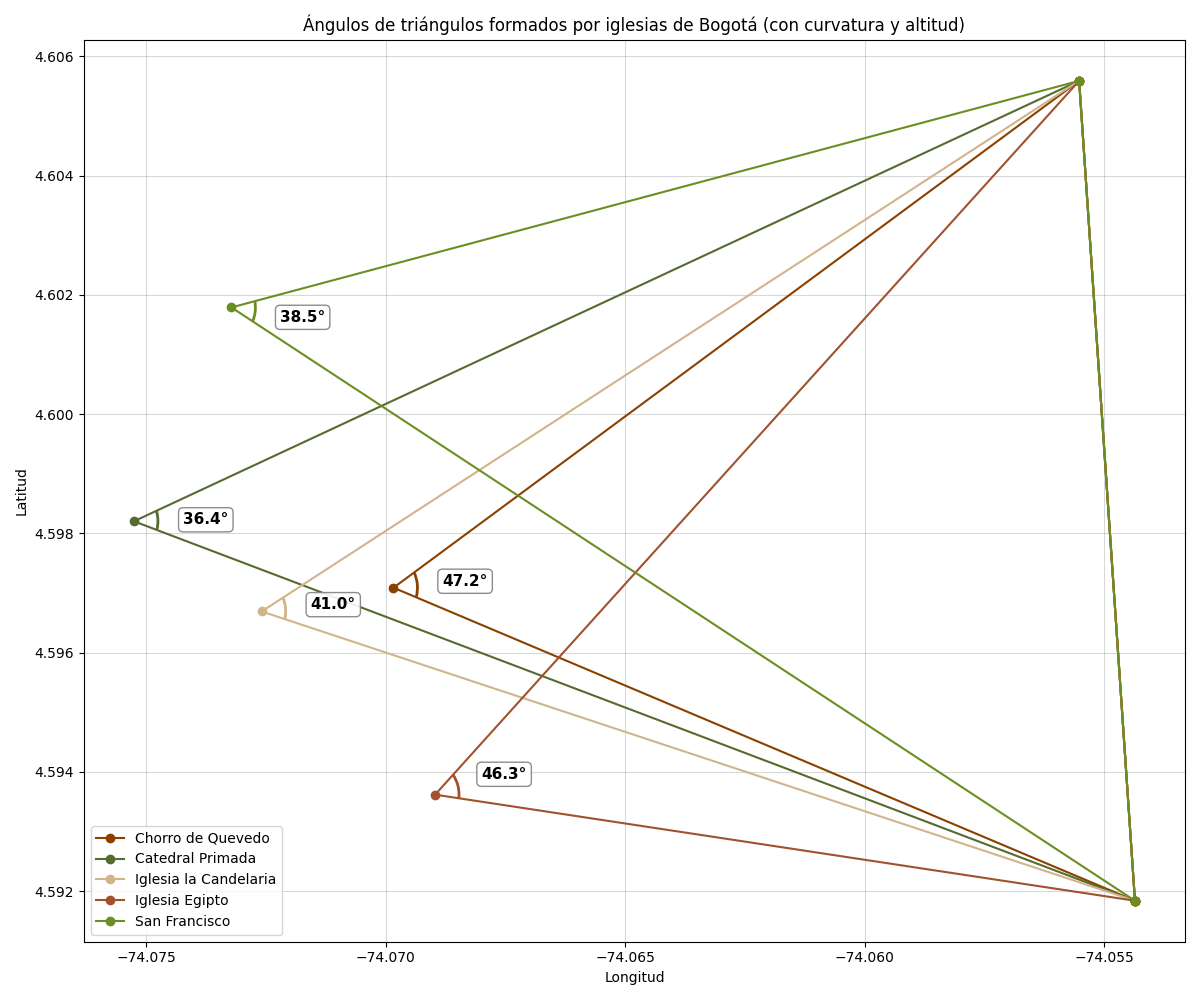
\includegraphics[width=0.45\textwidth]{images/triangles_with_arcs.png}
    \captionof{figure}{ Representacion  2D latitud y longitud de los triangulos de alineaciones solares. }

\justifying


\section{Resultados y analisis}
idea 1
los ángulos obtenidos en el cuadro 2 evidencian una alta correspondencia entre el cálculo teórico del punto de observación ideal del amanecer solar y la ubicación de la ermita de san miguel del principe, en el Chorro de Quevedo, este sitio considerado el lugar fundacional de la ciudad de Bogotá. La precisión del alineamiento sugiere que desde este punto es posible observar con gran cercanía la alineacion natural durante solsticios y equinoccios, lo que sugiere  que el punto de inicio de la ciudad no fue elegido al azar, sino que responde a criterios astronómicos o simbólicos asociados a la cosmovisión indígena.
idea 2
Curiosamente, el área del Chorro de Quevedo se encuentra próxima a una vía cuyo nombre histórico es la Calle del sol, hecho que adquiere relevancia al contrastarlo con la alineación calculada. Esta coincidencia entre la orientación astronómica y la toponimia urbana parece reflejar una continuidad simbólica entre el orden espacial colonial y la antigua observación del cielo.

En 1774, el virrey Manuel Guirior, el 10 de noviembre, ordenó la organización y denominación de las calles principales de Bacatá, instruyendo a los alcaldes locales para asignar nombres distintivos a cada una de ellas. Tal como señala Mejía (1999), “todo nombre de calles implicaba una asociación que permitía materializar en la mente de los habitantes una forma colectiva de percibir el espacio”. En este sentido, la existencia de una “Calle del sol” en las inmediaciones del punto fundacional puede interpretarse como un vestigio de esa práctica simbólica: una forma de inscribir en la ciudad una relación entre el espacio urbano y los fenómenos celestes.

idea 3
La catedral primada de bogota no posee la mejor alineacion respecto a os anculos teoricos ni tampoco un fuerte fundamento historico. Poe el contrario, El Chorro de Quevedo, además de ser reconocido como el punto donde se fundó la ciudad por Gonzalo Jiménez de Quesada, tuvo probablemente una función previa de carácter ritual o astronómico para las comunidades muiscas, quienes realizaban observaciones del Sol y la Luna desde puntos estratégicos del altiplano. Por su posición elevada y su visibilidad del horizonte oriental, el lugar habría facilitado la identificación de los ciclos lunares y solares, fundamentales en el calendario agrícola y ceremonial indígena.

Idea 4 

Area de observacion, inclusion de esta practica dentro de la actual cultura bogotana contemporanea

\section{Conclusions}
The proposed alignment process, detailed in   Sections
successfully aligns ALMA and IRIS images using the helioprojective coordinates from SDO as a reference point. The 


\section*{Acknowledgments}
This paper makes use of the following ALMA data: ADS/JAO.ALMA\#2017.1.00653.S. ALMA is a partnership of ESO (representing its member states), NSF (USA), and NINS (Japan), together with NRC (Canada), MOST and ASIAA (Taiwan), and KASI (Republic of Korea), in co-operation 




\bibliography{biblio}

\end{document}